% little trick to replace lib.tex by this
\renewcommand{\doctitle}[1]{
	\chapter{#1}
}
\renewcommand{\biblio}[1]{}
\doctitle{Dimensionnement du modulateur sigma-delta}

\section{Fonctionnement et théorie}
Le schéma bloc du modulateur sigma-delta se trouve
à la figure \ref{fig:sigma-delta-schema-blocs}. Ici,
on choisit une bascule asymétrique.

\begin{figure}[ht]
	\centering
	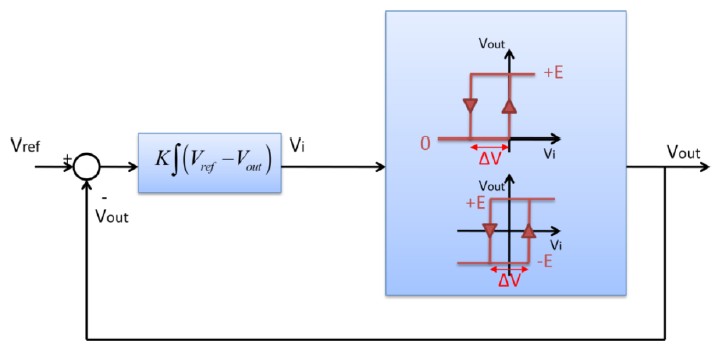
\includegraphics[scale=0.75]{img/schema-blocs.png}
	\caption{Schéma bloc du modulateur sigma-delta.}
	\label{fig:sigma-delta-schema-blocs}
\end{figure}

Dans un premier temps, calculons la période
d'oscillation de la sortie (qui est identique
à la période d'oscillation de $V_I$ sur la figure
\ref{fig:sigma-delta-schema-blocs}.

On démarre avec un signal $V_{\text{ref}}$ positif et
$V_{\text{out}} = 0$. $V_I$ est alors immédiatement positif
et $V_{\text{out}}$ sature directement à $E$. Comme $V_{\text{ref}}$
est $\leq E$, $V_I$ va maintenant décroître jusqu'à atteindre
$\Delta V$. A ce moment précis, on aura à nouveau $V_{\text{out}} = 0$
et donc $V_I$ va croître jusqu'à atteindre 0, et ainsi de suite.

Sur base de cela, on peut facilement calculer
le temps de descente $t_f$ et le temps de montée $t_r$
du signal $V_I$\footnote{Ce signal sera soit un signal triangulaire,
soit un signal en dents de scie, selon la valeur de $V_{\text{ref}}$.}.
On trouve facilement,
\[ t_f = -\frac{\Delta V}{(V_{\text{ref}} - E)K},\]
\[ t_r = \frac{\Delta V}{KV_{\text{ref}}}.\]
La période $T$ étant la somme du temps de descente et du temps
de montée, on trouve
\[ T = \frac{\Delta V}{K}\left(\frac{1}{V_{\text{ref}}} - \frac{1}{V_{\text{ref}} - E}\right)\]
et donc finalement
\[ f = -\frac{K}{\Delta V} \frac{V_{\text{ref}}(V_{\text{ref}}-E)}{E}.\]

\paragraph{Remarque}
A partir du temps de descente et du temps de montée, on
peut prouver que la moyenne du signal carré $V_{\text{out}}$
vaut bien $V_{\text{ref}}$. Il suffit de démontrer l'égalité
suivante
\[ \frac{E \cdot t_f + 0 \cdot t_r}{T} = V_{\text{ref}}.\]

La figure \ref{fig:sigma-delta-f-vs-vref} représente un
graphe de cette relation.

\begin{figure}[ht]
	\centering
	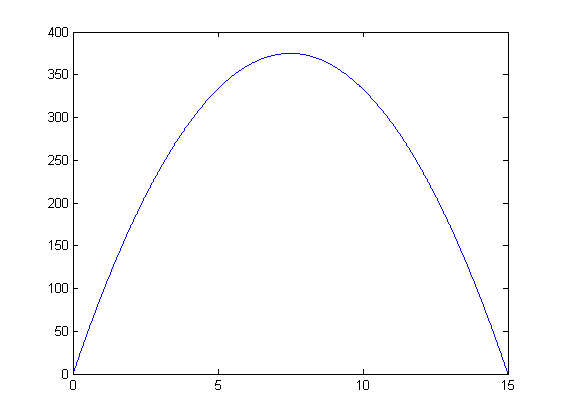
\includegraphics[scale=0.6]{img/sigma-delta-f-vs-vref.png}
	\caption{Graphe de la fréquence en fonction de $V_{\text{ref}}$
	pour $\Delta V$ = \unit{0.1}{\volt} et $K = \unit{10}{\second}$.}
	\label{fig:sigma-delta-f-vs-vref}
\end{figure}

On peut faire plusieurs observations à propos de la figure
\ref{fig:sigma-delta-f-vs-vref}. Premièrement, la fréquence
de sortie maximale est atteinte pour $V_{\text{ref}} = \frac{E}{2}$
et vaut
\[ f_{\text{max}} = \frac{K}{\Delta V}\frac{E}{4}. \]
Ensuite, pour un signal $V_{\text{ref}}$ sinusoïdal dont
l'amplitude peut être négative, la fréquence sature.
% FIX ME : je ne sais pas comment exprimer ça correctement.
Or, dans le cas de notre synthétiseur, le signal $V_{\text{ref}}$
est la sortie de notre VCO (après passage dans un filtre pour
en extraire une sinusoïdale pure).
Il faudra donc ``déplacer'' la courbe de la figure
\ref{fig:sigma-delta-f-vs-vref} de manière à ce qu'elle soit
centré autour de l'origine.

\section{Dimensionnement et circuit réel}
Le circuit du modulateur sigma-delta est représenté
à la figure \ref{fig:sigma-delta-circuit}.

\begin{figure}[ht]
	\centering
	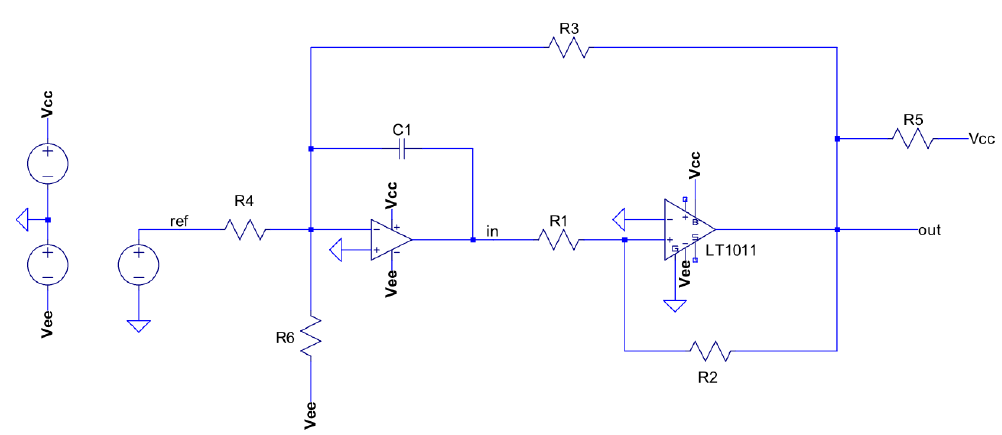
\includegraphics[scale=0.7]{img/sigma-delta-circuit.png}
	\caption{Circuit du modulateur.}
	\label{fig:sigma-delta-circuit}
\end{figure}

On va résoudre ce circuit pour obtenir des équations
de la même forme que celles de la figure
\ref{fig:sigma-delta-schema-blocs}.
On se concentre d'abord sur l'amplificateur
opérationnel. Grâce à la boucle de contre
réaction négative, on peut dire $v_- = v_+ = 0$.
On peut ensuite obtenir les courants suivants
\[ i_{R_4} = \frac{V_{\text{ref}}}{R_4},\]
\[ i_{R_6} = \frac{V_{\text{ee}}}{R_6},\]
\[ i_{R_3} = \frac{V_{\text{out}}}{R_3},\]
\[ i_{C_1} = -C_1\fdif{v_{\text{in}}}{t}.\]
On applique ensuite KCL et on écrit
\[ i_{C_1} = i_{R_4} + i_{R_6} + i_{R_3}.\]
De cette relation, on tire
\[ v_{\text{in}} = -\frac{1}{C_1}\int \frac{V_{\text{ref}}}{R_4}
+ \frac{V_{\text{ee}}}{R_6} + \frac{V_{\text{out}}}{R_3}.\]
Pour se ramener à l'équation de la figure
\ref{fig:sigma-delta-schema-blocs}, on pose
$V'_{\text{ref}} = -R_3(\frac{V_{\text{ref}}}{R_4}+\frac{V_{\text{ee}}}{R_6})$
pour enfin obtenir
\[ v_{\text{in}} = \frac{1}{C_1R_3} \int V'_{\text{ref}} - V_{\text{out}}\]
où $V'_{\text{ref}}$ correspond au $V_{\text{ref}}$
de la figure \ref{fig:sigma-delta-schema-blocs}.

Pour dimensionner le modulateur, on doit respecter plusieurs
contraintes. Premièrement la fréquence pour $V_{\text{ref}} =$
\unit{7.5}{\volt} doit être de \unit{80}{\kilo\hertz}. Et deuxièment,
on doit déplacer la courbe de la figure \ref{fig:sigma-delta-f-vs-vref}
de manière à ce que ces racines soient \unit{-15}{\volt} et
\unit{+15}{\volt}. Enfin, on doit choisir $\Delta V$ de manière
à ce que la bascule ne soit pas sensible au bruit (quelques millivolts).

On va directement anticiper une non-idéalité de la bascule,
la valeur de saturation $E$ n'est pas égale à la tension
d'alimention. On a plutôt $E \approx$ \unit{13.5}{\volt}.

Pour centrer la parabole, il faut que $\frac{R_3}{R_6}V_{\text{ee}}$
soit égale à \unit{6.75}{\volt}. Il faut ensuite étirer la
parabole de manière à ce que ses racines soient $\pm$\unit{15}{\volt}.
Il faut donc $\frac{R_3}{R_4} = 0.45$. 

En restant dans des valeurs de composants standards (série de Renard E12). 
On peut choisir, $R_3 =$ \unit{22}{\kilo\ohm} et $R_4 = R_6 =
$ \unit{47}{\kilo\ohm}.

On passe ensuite à la contrainte sur la fréquence. On a comme
relation 
\[ \frac{K}{\Delta V} = 30796.\]
On peut fixer arbitrairemet $\Delta V$ à \unit{1}{\volt}. On alors
$K = \frac{1}{C_1R_3} = 30796$ et donc $C1 =$ \unit{1.5}{\nano\farad}.
Enfin, comme $\Delta V = \frac{R_1}{R_2}E$, on peut par exemple
choisir $R_1 =$ \unit{10}{\kilo\ohm} et $R_2 =$ \unit{82+47}{\kilo\ohm}.

% TODO : remplacr avec les nouvelles valeurs (voir sigma.m)

\end{document}